%% P4 -- Supplementary material (separate file; excluded from the manuscript word count)
%% Build: pdflatex supplement ; bibtex supplement ; pdflatex supplement ; pdflatex supplement
\documentclass[preprint,12pt,authoryear]{elsarticle}

\usepackage{amsmath}
\usepackage{booktabs}
\usepackage{array}
\usepackage{graphicx}
\usepackage{url}

\setlength{\emergencystretch}{2em}

\renewcommand{\thesection}{S\arabic{section}}
\renewcommand{\thefigure}{S\arabic{figure}}
\renewcommand{\thetable}{S\arabic{table}}
\renewcommand{\theequation}{S\arabic{equation}}

\begin{document}

\begin{frontmatter}

\title{Supplementary material for ``A dimensionless verification floor for model assessment: which accuracy claims can an observational archive actually resolve?''}

\end{frontmatter}

\noindent This supplement carries the derivations, provenance detail, sensitivity protocol, archive diagnostics and code inventory that the manuscript refers to as S1--S7. It is a separate file and is excluded from the manuscript word count under the publisher's rule (only the manuscript file is counted; abstract, keywords, highlights, references and captions are excluded).

\section{Derivation and the non-central $t$ correction}
\label{sec:s1}

The criterion follows from requiring that a test of size $\alpha$ reject the null when the true difference equals the asserted magnitude $\delta$ with probability $1-\beta$. Let $\hat{d}$ be the domain-mean product--truth difference, $\sigma_d$ the standard deviation of the difference field and $n_{\mathrm{eff}}$ the effective number of independent samples, so that $\mathrm{SE}(\hat{d}) = \sigma_d/\sqrt{n_{\mathrm{eff}}}$. Under the normal approximation the two-sided rejection region is $|\hat{d}| > z_{1-\alpha/2}\,\sigma_d/\sqrt{n_{\mathrm{eff}}}$, and the power at a true difference $\delta$ is
\begin{equation}
1-\beta \;=\; \Phi_{\mathrm{N}}\!\left(\frac{\delta\sqrt{n_{\mathrm{eff}}}}{\sigma_d}-z_{1-\alpha/2}\right)
+ \Phi_{\mathrm{N}}\!\left(-\frac{\delta\sqrt{n_{\mathrm{eff}}}}{\sigma_d}-z_{1-\alpha/2}\right),
\label{eq:power}
\end{equation}
where $\Phi_{\mathrm{N}}$ is the standard normal distribution function. Setting the power to $0.80$ and solving for $\delta$ gives
\begin{equation}
\delta \;\ge\; \left(z_{1-\alpha/2}+z_{1-\beta}\right)\frac{\sigma_d}{\sqrt{n_{\mathrm{eff}}}}
\;=\; 2.802\,\frac{\sigma_d}{\sqrt{n_{\mathrm{eff}}}},
\label{eq:mde}
\end{equation}
with $2.802 = 1.959964 + 0.841621$, the sum of the two-sided 5\,\% critical value and the 80\,\% power quantile \citep{cohen1992power,lenth2001some}. The second term of Eq.~(\ref{eq:power}) is negligible for the values of interest: the relation $\delta\sqrt{n_{\mathrm{eff}}}/\sigma_d = z_{1-\alpha/2}+z_{1-\beta}$ holds to better than $0.1\,\%$ once $n_{\mathrm{eff}} > 20$. Dividing Eq.~(\ref{eq:mde}) by the claim gives the testability index of the manuscript, $\Phi = 2.802\,\sigma_d/(\mathrm{claim}\sqrt{n_{\mathrm{eff}}})$.

For small effective sample sizes the statistic is non-central $t$ with $\nu = n_{\mathrm{eff}}-1$ degrees of freedom rather than normal, and the constant required for 80\,\% power rises. Solving $\Pr[T'(\delta') > t_{1-\alpha/2,\nu}] = 0.80$ for the non-centrality $\delta'$ with \texttt{scipy.stats.nct} gives 2.95 at $n_{\mathrm{eff}} = 20$ ($+5\,\%$), 3.15 at 10 ($+12\,\%$), 3.76 at 5 ($+34\,\%$) and 8.55 at 2.41 ($+205\,\%$); for the sea-ice count of 325.2 it is 2.81 ($+0.3\,\%$), and for the three large counts the change is below $1\,\%$. Only regional biomass is materially affected: its exact constant would raise $\Phi$ from 2.71 to 8.27. The correction therefore strengthens the one $\Phi>1$ verdict to which it applies and leaves the three verifiable domains and the sea-ice interval unchanged.

The 80\,\% power is a convention. At 90\,\% power the constant becomes $1.960+1.282 = 3.242$, raising all floors by 16\,\%; at 70\,\% it becomes $1.960+0.524 = 2.484$, lowering them by 11\,\%. No verdict in the five-domain ranking changes under either alternative.

\section{Inputs, harmonisation and closure rules}
\label{sec:s2}

\subsection{Harmonisation}
\label{sec:s2a}

Three quantities must be established on a common footing before the criterion can be applied: $n_{\mathrm{eff}}$, $\sigma_d$ and the claimed magnitude. The rule is applied identically in all five domains: the difference field, the claim and the correlation model must refer to the same geophysical quantity, in the same units, averaged over the same space and time scale. A claim about instantaneous 9 km soil moisture cannot be tested against daily station values; a claim about monthly basin-mean ice thickness cannot be tested against individual flight transects; a claim about annual biomass carbon cannot be tested against single-footprint lidar returns. Where a published claim is phrased at a different scale from the available truth, it is re-expressed at the scale of the truth and the transformation is recorded rather than silently applied.

Table~\ref{tab:provenance} gives, for each domain, the raw count, the closure rule used to obtain $n_{\mathrm{eff}}$, the source of $\sigma_d$, the source of the claim and the resulting value. Every entry is traceable either to a peer-reviewed source or to a data product with a persistent identifier; entries that could not be traced are marked and excluded from the verdict rather than replaced by a plausible proxy. The sea-ice truth archive is documented by \citet{kurtz2013sea}, \citet{kurtz2011snow} and \citet{icebird_pangaea}; the soil-moisture network by \citet{dorigo2021international} and \citet{gruber2018sparse}; the precipitation gauges by \citet{gpcc_v2022}; and the biomass plots by \citet{duncanson2022aboveground}.

\begin{table}[t]
\caption{Provenance of the three quantities that enter the criterion, by domain. ``Rule'' is the closure used to convert the raw count into $n_{\mathrm{eff}}$; the corresponding algebra is given in Sect.~\ref{sec:s2b}. The last two rows are reported for completeness and are not used in any verdict, because at least one of their three quantities could not be traced to a verifiable source.}
\label{tab:provenance}
\scriptsize
\setlength{\tabcolsep}{3pt}
\begin{tabular}{>{\raggedright\arraybackslash}p{2.1cm}>{\raggedright\arraybackslash}p{1.9cm}>{\raggedright\arraybackslash}p{2.2cm}>{\raggedright\arraybackslash}p{2.4cm}>{\raggedright\arraybackslash}p{1.7cm}>{\raggedright\arraybackslash}p{1.4cm}}
\toprule
Domain & Raw count & Rule for $n_{\mathrm{eff}}$ & $\sigma_d$ (source) & Claim (source) & $n_{\mathrm{eff}}$ \\
\midrule
Sea-ice thickness & 40\,084 ATM L1B granules, 2009--2019; 338 flight days & Sortie capacity: one independent segment per flight day at $L = 326$ km; 297 days plus 28.2 from IceBird 2019 & 0.65 m, measured CCI--IceBird/ATM difference, range 0.50--0.80 m & 0.027 m, 2\,\% of 1.36 m mean, mask-induced bias & 325.2 \\
Soil moisture & 2\,842 stations in 71 networks (ISMN, July 2021) & Cluster design effect, $m = 40$ stations per network, $\rho = 0.5$ & 0.040 m$^3$ m$^{-3}$, SMAP ubRMSE target and observed & 0.040 m$^3$ m$^{-3}$, mission accuracy (ubRMSE) & 138.6 \\
Sea-surface salinity & $\sim$1.56 $\times$ 10$^6$ Argo profiles over 10 years; 13\,000 per month & Area $\times$ time: $A/(2\pi L^2)\cdot T/\tau$ with $A = 3.6\times10^8$ km$^2$, $L = 333$ km, $\tau = 3$ months & 0.20 PSU, SMAP--buoy SD of 0.22 weekly and 0.17 monthly & 0.20 PSU, mission accuracy & 20\,668 \\
Precipitation & 50\,000 gauges in the Chinese automatic network; 78\,000 in GPCC & Area $\times$ time: $A = 9.6\times10^6$ km$^2$, $L = 100$ km, $T = 1095$ d, \mbox{$\tau = 3$ d} & 3.0 mm d$^{-1}$, order of the daily IMERG--gauge difference & 0.82 mm d$^{-1}$, 20\,\% of the 4.1 mm d$^{-1}$ mean & 55\,768 \\
Forest biomass & 39 plots in one region; 74\,860 GEDI L4A granules & Cluster design effect, $m = 39$, $\rho = 0.4$ & 45 Mg ha$^{-1}$, literature RMSE 39--94, median 45 & 30 Mg ha$^{-1}$, 20\,\% of the 150 Mg ha$^{-1}$ mean & 2.41 \\
\midrule
Forest biomass, global & GEDI L4A 74\,860 granules; $\sim$8\,000 plots reported & Cluster, $m = 30$, $\rho = 0.5$ & as above & as above & 516 (not assessable) \\
Snow depth on sea ice & 174\,799 OIB snow-radar granules; 297 flight days & none: the product uses the same radar & 0.10 m, magnitude cited, not audited & 0.05 m, bias claim & not assessable \\
\bottomrule
\end{tabular}
\end{table}

Two domains were examined and set aside under the traceability rule. A global biomass variant, at about 8\,000 plots with $m = 30$ and $\rho = 0.5$, would give $n_{\mathrm{eff}} = 516$ and $\Phi = 0.18$, but neither the plot count nor the number of plots outside the GEDI training set could be verified from public documentation. Snow depth on sea ice fails a different test: the product and the truth share the same snow radar, so the comparison is not independent and $n_{\mathrm{eff}}$ has no meaning in the intended sense.

\subsection{Closure rules}
\label{sec:s2b}

Three closures were used. For clustered truth, the single-level form of the Kish design effect is
\begin{equation}
n_{\mathrm{eff}} = \frac{n}{1+(m-1)\rho},
\label{eq:cluster}
\end{equation}
where $m$ is the cluster size and $\rho$ the intra-cluster correlation. For soil moisture, $n = 2\,842$, $m = 2\,842/71 \approx 40$ and $\rho = 0.5$, giving 138.6; the strict 18-site variant uses $n = m = 18$ and gives 18, hence $\Phi = 0.66$. For regional biomass, $n = m = 39$ and $\rho = 0.4$, giving 2.41.

For truth distributed over an area with correlation length $L$ and over a time window $T$ with correlation time $\tau$, the number of decorrelation cells is
\begin{equation}
n_{\mathrm{eff}} = \frac{A}{2\pi L^{2}}\,\frac{T}{\tau},
\label{eq:area}
\end{equation}
the factor $2\pi$ rather than $4$ reflecting the Gaussian rather than boxcar form of the decorrelation cell \citep{bretherton1999effective,zwiers1995taking,kish1965survey}. For salinity, $A = 3.6\times10^{8}$ km$^2$, $L = 333$ km, $T = 120$ months and $\tau = 3$ months give 20\,668. For precipitation, $A = 9.6\times10^{6}$ km$^2$, $L = 100$ km, $T = 1095$ days and $\tau = 3$ days give 55\,768.

For truth that arrives as transects, capacity is set by the number of independent segments per sortie,
\begin{equation}
n_{\mathrm{seg}} = \max\!\left(1, \frac{\ell}{2L}\right),
\label{eq:sortie}
\end{equation}
summed over sorties, with $\ell$ the typical sortie length. With $\ell \approx 450$ km and $L = 326$ km each sortie contributes one segment; 297 flight days plus 28.2 from IceBird give 325.2. The factor of two in the denominator is the same one that appears in Eq.~(\ref{eq:area}) and reflects the two-sided nature of a correlation length.

\section{The kernel family}
\label{sec:s3}

The extended sea-ice record supports two correlation models of the difference field \citep{ricker2017weekly,sallila2019assessment}, both defensible, whose floors differ by a factor of three (Fig.~\ref{fig:kernel}). The first is an exponential kernel with $L = 326$ km fitted to the product's own spatial variability, which yields 10.38 cm for the archive design with eight sorties per campaign. The second is the empirical autocorrelation of the product--truth difference itself, whose measured values are $\rho(25\,\mathrm{km}) = 0.269$, $\rho(75\,\mathrm{km}) = 0.080$ and $\rho(150\,\mathrm{km}) \approx 0$; because the difference decorrelates four times faster than the field, the same archive yields 3.447 cm.

\begin{figure}[t]
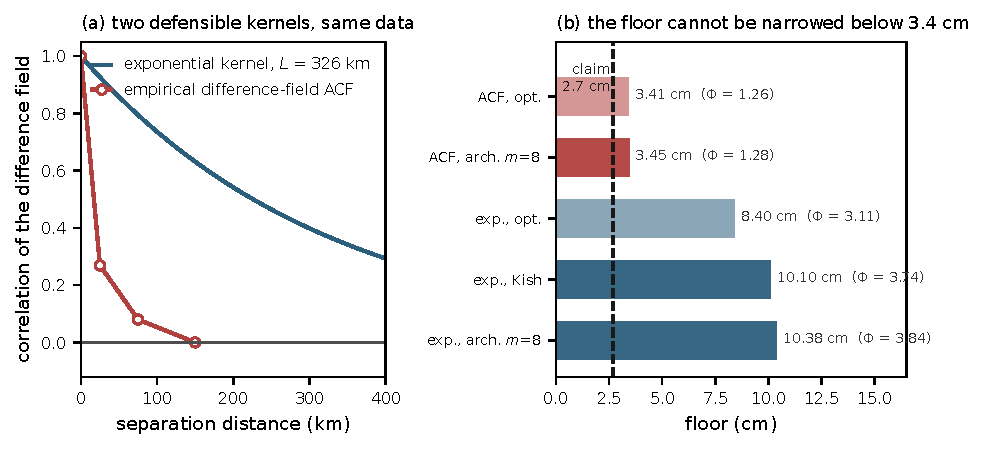
\includegraphics[width=\textwidth]{figures/fig5_kernel.pdf}
\caption{(a) Two correlation models of the same difference field. The exponential kernel with $L = 326$ km describes the spatial variability of the thickness field; the empirical autocorrelation of the product--truth difference falls to 0.269 at 25 km and to zero by 150 km. (b) The verification floor implied by each kernel under the design assumptions of Table~\ref{tab:kernel}. The claim is 2.7 cm. The floor ranges from 3.406 to 10.38 cm, a factor of 2.5 between the respective optima and of 3.0 at fixed archive design; $\Phi$ therefore cannot be quoted as a single number.}
\label{fig:kernel}
\end{figure}

The ambiguity cannot be removed by collecting more data, and that is the point. The two kernels answer different questions: the exponential kernel describes how much independent information the field contains, the empirical kernel how much independent information the difference contains. Both are legitimate, neither is a mistake, and which one is appropriate depends on whether the claim is about the field's representativeness or about the retrieval's systematic error. A validation study that adopted one silently would report a floor that another equally careful study could dispute by a factor of three, with no datum able to settle the dispute. The kernel choice is therefore treated as a Methods-level commitment, both results are stated wherever the sea-ice number appears, and $\Phi$ is reported as the interval spanned by the two floors.

Two further design variants close the space. If the archive is optimised -- roughly eight sorties per campaign concentrated in the months that matter -- the exponential kernel gives 8.40 cm and the empirical kernel 3.406 cm, a factor of 2.5. If instead each campaign contributes 27 sorties, the exponential kernel gives 10.38 cm ($\Phi = 3.84$). Table~\ref{tab:kernel} lists the five members of the family with their floors and $\Phi$ values. The complete family spans 3.406--10.38 cm; the interval quoted in the manuscript, 3.447--10.098 cm ($\Phi = 1.28$--$3.74$, reported as 1.3--3.7), is the sub-family of physically realised designs, anchored to the Kish equal-weight count used for every other domain. Every member lies above the 2.7 cm claim: the verdict is kernel-independent even though the number is not.

\begin{table}[t]
\caption{The sea-ice floor as a function of correlation kernel and archive design. ``Optimised'' is the allocation of roughly eight sorties per campaign; ``Kish archive'' is the equal-weight count of 297 flight days plus IceBird; ``archive $m = 8$'' is the realised design with eight sorties per campaign. $\Phi$ is the floor divided by the 2.7 cm claim.}
\label{tab:kernel}
\footnotesize
\setlength{\tabcolsep}{4pt}
\begin{tabular}{llccc}
\toprule
Kernel & Design & Floor (cm) & $\Phi$ \\
\midrule
Empirical difference-field ACF & Optimised & 3.406 & 1.26 \\
Empirical difference-field ACF & Archive, $m = 8$ & 3.447 & 1.28 \\
Exponential, $L = 326$ km & Optimised & 8.40 & 3.11 \\
Exponential, $L = 326$ km & Kish archive & 10.098 & 3.74 \\
Exponential, $L = 326$ km & Archive, $m = 8$ & 10.38 & 3.84 \\
\bottomrule
\end{tabular}
\end{table}

\section{Sensitivity protocol and grids}
\label{sec:s4}

Each of $\sigma_d$ and the claim was perturbed by $\pm 50\,\%$ in five steps, giving a 25-cell grid per domain, and the same grid was applied to the two sea-ice kernel bounds and to the strict 18-site soil-moisture variant. Two summaries are reported: the axis-wise range, in which one quantity varies while the other is held at its nominal value, and the joint range over the full box. The $\pm 50\,\%$ width was chosen because it exceeds the spread of the published $\sigma_d$ values in three of the five domains (0.50--0.80 m for sea ice, 39--94 Mg ha$^{-1}$ for biomass, 0.17--0.22 PSU for salinity) and because it brackets the plausible range of a claim that is itself stated as an order-of-magnitude target. Because $\Phi$ is linear in $\sigma_d$ and inverse-linear in the claim, the sensitivity is analytic and requires no simulation; the grids in Fig.~\ref{fig:sensitivity} are computed directly from the criterion.

\begin{figure}[t]
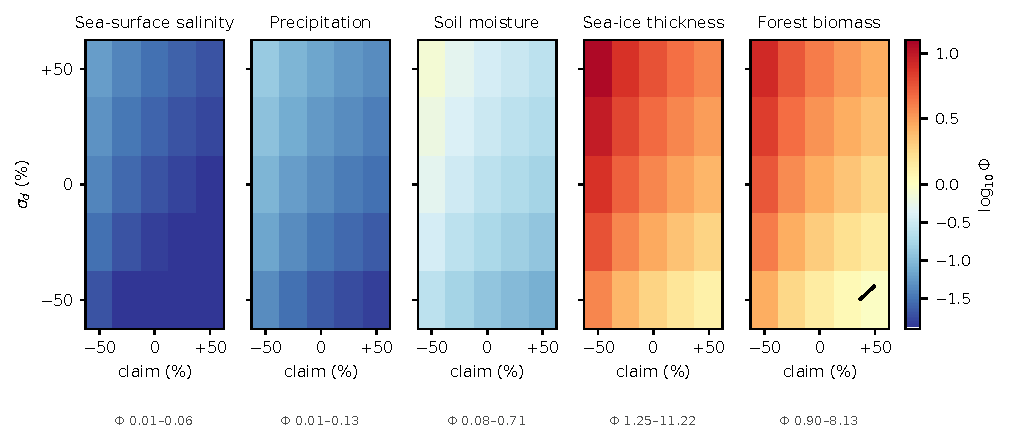
\includegraphics[width=\textwidth]{figures/fig4_sensitivity.pdf}
\caption{Sensitivity of $\Phi$ to $\pm 50\,\%$ perturbations of $\sigma_d$ (vertical axis) and of the claim (horizontal axis). Colour is $\log_{10}\Phi$ with white at $\Phi = 1$; the black contour in the biomass panel is the $\Phi = 1$ line and the ranges printed below each panel are the minima and maxima over the 25-cell grid. Salinity, precipitation and soil moisture never approach the watershed; sea ice at its exponential-kernel bound never crosses it; biomass and the empirical-kernel sea-ice bound do.}
\label{fig:sensitivity}
\end{figure}

\begin{table}[t]
\caption{Sensitivity summary. ``Axis-wise'' varies one quantity at a time over $\pm 50\,\%$; ``joint'' is the full 25-cell box. The two rows below the rule give the alternative sea-ice kernel bound and the strict 18-site soil-moisture variant, which are kept out of the main ranking but bear on its robustness.}
\label{tab:sensitivity}
\footnotesize
\setlength{\tabcolsep}{3pt}
\begin{tabular}{@{}>{\raggedright\arraybackslash}p{2.6cm}ccc>{\raggedright\arraybackslash}p{2.2cm}@{}}
\toprule
Domain & $\Phi$ nominal & Axis-wise range & Joint range & Robustness \\
\midrule
Sea-surface salinity & 0.019 & 0.0097--0.039 & 0.0065--0.058 & robustly verifiable \\
Precipitation & 0.043 & 0.022--0.087 & 0.014--0.130 & robustly verifiable \\
Soil moisture & 0.24 & 0.119--0.476 & 0.079--0.714 & robustly verifiable \\
Sea-ice thickness (exponential) & 3.74 & 1.87--7.48 & 1.25--11.2 & robustly not verifiable \\
Forest biomass & 2.71 & 1.35--5.42 & 0.90--8.13 & flips at optimistic corner \\
\midrule
Sea-ice, empirical-kernel bound & 1.28 & 0.64--2.55 & 0.43--3.83 & flips at optimistic corner \\
Soil moisture, 18-site strict variant & 0.66 & 0.33--1.32 & 0.22--1.98 & flips \\
\bottomrule
\end{tabular}
\end{table}

The verdicts separate into three classes. Salinity, precipitation and soil moisture never approach unity anywhere in the box: their maxima are 0.058, 0.130 and 0.714, all at the corner where $\sigma_d$ is 50\,\% high and the claim 50\,\% low. Sea ice at its exponential-kernel bound never falls below unity: its minimum, at the opposite corner, is 1.25. Regional biomass reaches 0.90 at that corner, and so does sea ice at its empirical-kernel bound, which reaches 0.43. The asymmetry between the two sea-ice bounds is the most consequential result in the table: at the exponential bound the verdict is unperturbable inside the box, at the empirical bound a simultaneous 50\,\% reduction of $\sigma_d$ and 50\,\% increase of the claim would bring the criterion below unity. The sea-ice verdict therefore survives only under the conservative kernel, which is falsification condition F1 of the manuscript.

\section{The archive measurement}
\label{sec:s5}

For sea ice the effective sample size can be measured rather than assumed. The monthly CCI thickness field is subtracted from the monthly CS2SMOS field cell by cell on the common 25 km grid, wherever both products are defined -- about 18\,000 of the $432\times432$ cells for a typical April -- and the standard deviation of that difference is taken for each of the 43 winter months in which the products overlap, 2011--2024. The median monthly $\sigma_d$ is 0.389 m, the range 0.284--0.552 m and the root-mean-square 0.461 m. Two features of this measurement are carried into the manuscript: CCI and CS2SMOS both ingest CryoSat-2, so a mask-related difference is common to both and cancels in part, which makes 0.389 m the optimistic end and the independent airborne 0.65 m the conservative end; and the monthly value varies by season, from 0.326 m in November to 0.500 m in April.

The same difference field gives the correlation structure. Along each grid axis the empirical autocorrelation is computed to 30 lags (750 km), the bandwidth factor
\begin{equation}
\kappa = 1 + 2\sum_{k=1}^{K}\rho(k)
\label{eq:kappa}
\end{equation}
is formed with the sum truncated at the first non-positive value, and the valid cell count is divided by $\kappa_x\kappa_y$. For 2019-04, $\kappa_x = 7.69$ and $\kappa_y = 7.07$ over 18\,033 cells give $n_{\mathrm{eff}} = 331.8$. Table~\ref{tab:months} lists the four months quoted in the manuscript; April months give 311--394 and November 150, so the effective count has a seasonal floor. Fig.~\ref{fig:acf} shows the 2019-04 autocorrelation along both axes, with bandwidths of 192 and 177 km.

\begin{table}[t]
\caption{Measured diagnostics for the four months quoted in the manuscript. $n_{\mathrm{valid}}$ is the number of cells where both products are defined; $\kappa_x$ and $\kappa_y$ are the bandwidth factors of Eq.~(\ref{eq:kappa}); the bandwidths are $2\pi$-equivalent decorrelation lengths along each axis; $n_{\mathrm{eff}} = n_{\mathrm{valid}}/(\kappa_x\kappa_y)$; $\sigma_d$ is the monthly standard deviation of the CCI--CS2SMOS difference.}
\label{tab:months}
\footnotesize
\setlength{\tabcolsep}{4pt}
\begin{tabular}{lccccccc}
\toprule
Month & $n_{\mathrm{valid}}$ & $\kappa_x$ & $\kappa_y$ & $L_x$ (km) & $L_y$ (km) & $n_{\mathrm{eff}}$ & $\sigma_d$ (m) \\
\midrule
2018-04 & 18\,173 & 7.400 & 6.226 & 185.0 & 155.7 & 394.4 & 0.483 \\
2019-04 & 18\,033 & 7.686 & 7.071 & 192.2 & 176.8 & 331.8 & 0.500 \\
2020-11 & 13\,307 & 9.612 & 9.253 & 240.3 & 231.3 & 149.6 & 0.326 \\
2021-04 & 18\,189 & 8.085 & 7.238 & 202.1 & 181.0 & 310.8 & 0.463 \\
\bottomrule
\end{tabular}
\end{table}

\begin{figure}[t]
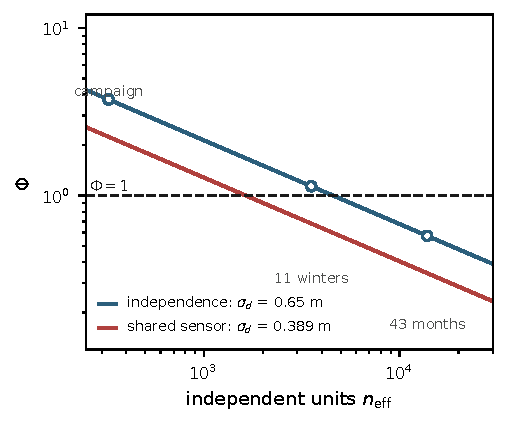
\includegraphics[width=0.62\textwidth]{figures/fig6_design.pdf}
\caption{$\Phi$ against independent units $n_{\mathrm{eff}}$ for the two ends of the measured $\sigma_d$: 0.389 m (shared CryoSat-2 sampling) and 0.65 m (independent airborne truth). The dashed line is $\Phi = 1$; markers are the campaign design, the fourteen-winter archive (one independent month each) and the 43-month pooled upper bound. The crossing sits between 1\,631 and 4\,550 independent units, so the binding quantity is archive length rather than the 2.7 cm claim.}
\label{fig:design}
\end{figure}

The measured count agrees with the design value 325.2 to 2\,\%, and that is all the agreement supports: the sortie-capacity closure is not arbitrary, but neither has the criterion been validated. What the archive changes is the verdict. Fourteen winters, one independent month each, give $n_{\mathrm{eff}} = 4\,498$; 43 pooled months give 13\,816, an upper bound because the pooling assumes no interannual correlation. With the measured $\sigma_d$ the campaign $\Phi$ falls from 2.24 to 0.60; with the independent airborne 0.65 m it falls from 3.74 to 1.006, from not verifiable to exactly at the boundary. The archive reaches $\Phi < 1$ at $n_{\mathrm{eff}} > 1\,631$ if $\sigma_d = 0.389$ m, and at $n_{\mathrm{eff}} > 4\,550$ if $\sigma_d = 0.65$ m.

\begin{figure}[t]
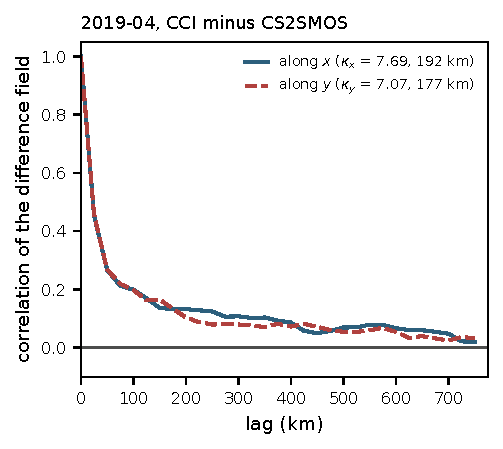
\includegraphics[width=0.62\textwidth]{figures/fig7_acf.pdf}
\caption{Autocorrelation of the 2019-04 CCI--CS2SMOS difference field along $x$ (solid) and $y$ (dashed), to 30 lags. The bandwidth factors are $\kappa_x = 7.69$ and $\kappa_y = 7.07$, and the corresponding decorrelation lengths are 192 and 177 km.}
\label{fig:acf}
\end{figure}

\section{Four diagnostics}
\label{sec:s6}

Four numbers in the calculation are worth isolating because they are not usually reported in validation papers. The first is the information collapse factor $n/n_{\mathrm{eff}}$, which is 123 for sea ice, 20.5 for soil moisture, 16.2 for biomass, 75 for salinity and 0.90 for precipitation. A paper that reports 40\,084 granules has, for the question at hand, 325 samples; a paper that reports 50\,000 gauges has 55\,768. The second is the floor in absolute units -- 10.1 cm of ice, 0.0095 m$^3$ m$^{-3}$ of soil moisture, 0.0039 PSU of salinity, 0.036 mm d$^{-1}$ of precipitation and 81 Mg ha$^{-1}$ of biomass -- which converts an abstract ratio into a statement a reader can judge. The third is the sample size that would be required to verify the current claim, $n_{\mathrm{eff}}\Phi^{2}$, which is 4\,550 for sea ice, 17.7 for biomass, 7.85 for soil moisture and 105 for precipitation. The fourth is the claim that would be verifiable with the present archive, $\mathrm{MDE}_{80}$, which answers the question ``what may we legitimately assert?''.

These four numbers turn a verdict into a research agenda, and the agendas differ by domain. Sea ice needs either a coarser claim or a truth that can be averaged at the product's footprint; biomass needs more independent plots, not better plots; soil moisture needs either denser networks or a claim stated at the scale the networks can support; salinity and precipitation need nothing except to keep making the claims they make. The criterion does not tell any of these domains to stop working. It tells each of them what kind of work would make its claims testable.

\section{Code structure and reproduction}
\label{sec:s7}

Because the method is arithmetic on published inputs, its example implementation is short and complete, and it is part of the submission rather than an illustration of it. The core implementation has two modules. \texttt{code/phi\_core.py} holds the three closures of Sect.~\ref{sec:s2b}, the constant of Eq.~(\ref{eq:mde}), the five domain records of Table~\ref{tab:provenance} and the kernel family of Table~\ref{tab:kernel}; it evaluates the criterion and writes the seven derived tables in \texttt{data/}. \texttt{code/run\_all.py} is the entry point: it runs the arithmetic, compares every headline number against the value printed in the manuscript and fails if any moves by more than 0.1\,\%, regenerates the seven figures in \texttt{figures/}, and builds both PDFs. A third script, \texttt{code/verify\_refs.py}, resolves the bibliography against Crossref and DataCite and is run on demand because it needs network access.

No observational granule is downloaded and no number is typed by hand: the five values of $\Phi$, the five kernel floors, the 25-cell sensitivity grids and the ranking figure are all generated from a single input table. Table~\ref{tab:provenance} is a transcription of that table. The implementation therefore serves three functions that a methods paper requires: it states the method unambiguously, it reproduces every reported number, and it can be applied to a new domain by adding one row to the input table.

The implementation is an example, not a general-purpose library. For the five domain records it does not acquire data, estimate a correlation function, or choose a claim; those three inputs remain the responsibility of the assessor, and the method is deliberately silent about how they should be obtained. A separate worked example, \texttt{code/archive\_example.py}, takes the one step that the five records leave open: it forms the cell-level difference of two real product fields, estimates the autocorrelation of that difference along each grid axis, and reports the resulting $n_{\mathrm{eff}}$ and $\Phi$, so that the step from a product pair to an $n_{\mathrm{eff}}$ is shown rather than asserted. It is an example of that step and not a recommendation of a single estimator.

The inventory is:

\begin{itemize}
\footnotesize
\item \texttt{code/phi\_core.py} -- constants, three closures, five domain records, kernel family, sensitivity grids; writes \texttt{data/*.csv}.
\item \texttt{code/make\_figures.py} -- the seven figures, read from \texttt{data/*.csv}.
\item \texttt{code/archive\_example.py} -- optional worked example on two monthly fields supplied from outside the archive.
\item \texttt{code/run\_all.py} -- one-command chain: arithmetic, number check, figures, both PDFs.
\item \texttt{code/test\_phi\_core.py} -- nine regression tests (\texttt{python -m pytest code}).
\item \texttt{code/verify\_refs.py} -- DOI/title audit of \texttt{refs.bib} (network).
\item \texttt{data/} -- seven derived tables plus the three committed tables that summarise the third-party archive.
\item \texttt{figures/} -- seven figure PDFs and PNG previews.
\item \texttt{manuscript.tex}, \texttt{supplement.tex}, \texttt{refs.bib} -- the two documents and the shared bibliography.
\end{itemize}

The script exits non-zero if a headline number moves by more than 0.1\,\% from the value printed in the manuscript, and the transcript of a reference run is recorded in \texttt{REPRO\_CHECK.txt}.

\bibliographystyle{elsarticle-harv}
\bibliography{refs}

\end{document}
